\needspace{10\baselineskip}
\begin{center}
\pdfbookmark[1]{10. Zu Art. 140.}{zusatz-010}
[10. Zu Art. 140.]
\end{center}
I. Es seien \(\mathfrak{A},\mathfrak{A}',\mathfrak{A}''\) die Abstände der drei Punkte \(A,A',A''\) von dem grössten Kreise \(BB^*B''\); \(h\) die Neigung dieses grössten Kreises gegen die Ekliptik, und \(H\) die Länge seines aufsteigenden Knotens auf der Ekliptik. Man hat dann
\[
\begin{aligned}
\sin\mathfrak{A}&=\sin h\sin(l-H)\\
\sin\mathfrak{A}'&=\sin h\sin(l'-H)\\
\sin\mathfrak{A}''&=\sin h\sin(l''-H),
\end{aligned}
\]
woraus leicht mit Hülfe des Lemma I in Art. 78 folgt:
\[
\begin{aligned}
1)\quad &\sin\mathfrak{A}\sin(l''-l')+\sin\mathfrak{A}'\sin(l-l'')\\
&\qquad+\sin\mathfrak{A}''\sin(l'-l)=0.
\end{aligned}
\]

II. Es seien ferner \(B,B^*,B''\) die Winkel, welche der grösste Kreis \(BB^*B''\) mit \(AB,A'B^*,A''B''\) macht, wodurch
\[
\begin{aligned}
\sin\mathfrak{A}&=\sin\delta\sin B\\
\sin\mathfrak{A}'&=\sin(\delta'-\sigma)\sin B^*\\
\sin\mathfrak{A}''&=\sin\delta''\sin B''.
\end{aligned}
\]

\SourceLeaf{311}
Die Gleichung 1 erhält demnach folgende Gestalt:
\[
\begin{aligned}
2)\quad &\sin\delta\sin B\sin(l''-l')\\
&\quad+\sin(\delta'-\sigma)\sin B^*\sin(l-l'')\\
&\quad+\sin\delta''\sin B''\sin(l'-l)=0.
\end{aligned}
\]

III. Man hat ferner
\[
\left.\begin{aligned}
A''D'-\delta''&=B''D'\\
AD'-\delta&=BD'\\
\frac{\sin B''D'}{\sin BD'}&=\frac{\sin B}{\sin B''}
\end{aligned}\right\}
\quad\text{folglich}\quad a=\frac{R\sin\delta\sin B}{R''\sin\delta''\sin B''}
\]
und
\[
3)\qquad \sin\delta\sin B=\frac{aR''\sin\delta''\sin B''}{R}\mathpunct{\raisebox{.45ex}{,}}
\]
wie auch
\[
\left.\begin{aligned}
A''D-\delta''&=B''D\\
A'D-\delta'+\sigma&=B^*D\\
\frac{\sin B''D}{\sin B^*D}&=\frac{\sin B^*}{\sin B''}
\end{aligned}\right\}
\quad\text{folglich}\quad b=\frac{R'\sin\delta'\sin B^*}{R''\sin\delta''\sin B''}
\]
und
\[
4)\qquad \sin B^*=\frac{bR''\sin\delta''\sin B''}{R'\sin\delta'}\mathpunct{\cdot}
\]

Diese Werthe aus 3, 4 in 2 substituirt geben eine Gleichung, die bei näherer Betrachtung mit der ersten Gleichung am Schluss von Art. 140 identisch gefunden wird.

IV. Um zum Beweise der andern Formel zu gelangen, sei \(P\) der Pol der Ekliptik, \(H\) der Punkt der Ekliptik, dessen Länge oben mit demselben Buchstaben bezeichnet wurde, also mit \(BB''\) in Einem grössten Kreise,
\[
\begin{aligned}
\text{also}\qquad HP&=90^0\\
BP&=90^0-\beta\\
B''P&=90^0-\beta''\\
BHP&=90^0-h\\
BPB''&=\alpha''-\alpha;
\end{aligned}
\]
\begin{center}
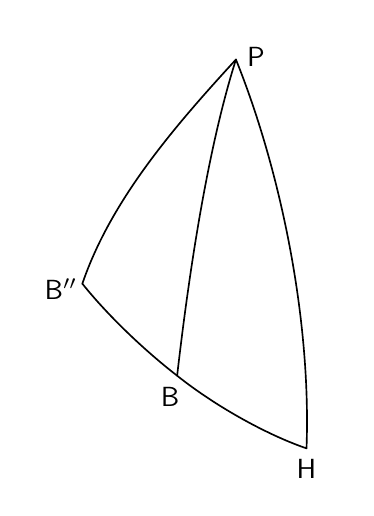
\begin{tikzpicture}[x=.25pt,y=-.25pt,line width=.6pt,line cap=round,line join=round]
\path[use as bounding box] (1850,2220) rectangle (2310,2885);
\draw (2151,2266)..controls(2060,2365)and(1970,2470)..(1929,2590);
\draw (1929,2590)..controls(1965,2635)and(2017,2685)..(2066,2723)..controls(2125,2770)and(2200,2810)..(2253,2828);
\draw (2253,2828)..controls(2260,2640)and(2215,2425)..(2151,2266);
\draw (2151,2266)..controls(2110,2395)and(2083,2575)..(2066,2723);
\node[inner sep=0pt,font=\fontsize{10}{11}\selectfont] at (2180,2262) {\(\mathsf{P}\)};
\node[inner sep=0pt,font=\fontsize{10}{11}\selectfont] at (1898,2598) {\(\mathsf{B}''\)};
\node[inner sep=0pt,font=\fontsize{10}{11}\selectfont] at (2056,2753) {\(\mathsf{B}\)};
\node[inner sep=0pt,font=\fontsize{10}{11}\selectfont] at (2253,2858) {\(\mathsf{H}\)};
\end{tikzpicture}
\end{center}
\[
\sin HB''P=\frac{\cos\beta\sin(\alpha''-\alpha)}{\sin BB''}\quad\text{(im Dreieck }BPB''\text{)}
\]
\[
\sin HB''P=\frac{\cos h}{\cos\beta''}\quad\text{(in dem Dreieck }HB''P\text{),}
\]
folglich
\[
5)\qquad \sin(\alpha''-\alpha)=\frac{\sin BB''\mathbin{.}\cos h}{\cos\beta\cos\beta''}\mathpunct{\cdot}
\]

Nun ist nach Art. 138, (7),
\[
S=\operatorname{tang}\beta\sin(\alpha''-l')-\operatorname{tang}\beta''\sin(\alpha-l'),
\]
\SourceLeaf{312}
also, da leicht zu übersehen ist, dass
\[
\operatorname{tang}\beta=\operatorname{tang}h\sin(\alpha-H),\quad\operatorname{tang}\beta''=\operatorname{tang}h\sin(\alpha''-H):
\]
\[
\begin{aligned}
S=\operatorname{tang}h\{&\sin(\alpha''-l')\sin(\alpha-H)\\
&-\sin(\alpha-l')\sin(\alpha''-H)\}
\end{aligned}
\]
oder, da nach Lemma I Art. 78 (wenn dort statt \(A,B,C\ldots\ \alpha-l',\alpha''-l',H-l'\) gesetzt wird) identisch ist
\[
\begin{aligned}
&\sin(\alpha-H)\sin(\alpha''-l')+\sin(H-\alpha'')\sin(\alpha-l')\\
&\qquad+\sin(\alpha''-\alpha)\sin(H-l')=0:
\end{aligned}
\]
\[
S=\operatorname{tang}h\sin(\alpha''-\alpha)\sin(l'-H),
\]
oder, für \(\sin(\alpha''-\alpha)\) den Werth aus 5 substituirt,
\[
6)\qquad S=\frac{\sin h\sin(l'-H)\sin BB''}{\cos\beta\cos\beta''}=\frac{\sin\mathfrak{A}'\sin BB''}{\cos\beta\cos\beta''}\mathpunct{\cdot}
\]

V. Wir haben ferner
\[
\sin\mathfrak{A}'=\sin AB^*\mathbin{.}\sin B^*=\sin(\delta'-\sigma)\sin B^*.
\]

Es ist also (Schluss von Art. 140)
\[
U=\frac{S}{\sin(\delta'-\sigma)}=\frac{\sin B^*\sin BB''}{\cos\beta\cos\beta''}
\]
oder da
\[
\sin BB'':\sin BD'=\sin\epsilon':\sin B'',
\]
d. i.
\[
\sin BB''=\frac{\sin(AD'-\delta)\sin\epsilon'}{\sin B''}:
\]
\[
U=\frac{\sin(AD'-\delta)\sin\epsilon'\sin B^*}{\cos\beta\cos\beta''\sin B''}
\]
oder
\[
\frac{\sin B^*}{\sin B''}=\frac{U\cos\beta\cos\beta''}{\sin(AD'-\delta)\sin\epsilon'}\mathpunct{\cdot}
\]

Dies in der obigen Gleichung \(b=\dfrac{R'\sin\delta'\sin B^*}{R''\sin\delta''\sin B''}\) substituirt, gibt
\[
b=\frac{R'\sin\delta'}{R''\sin\delta''}\cdot\frac{U\cos\beta\cos\beta''}{\sin(AD'-\delta)\sin\epsilon'}\mathpunct{\raisebox{.45ex}{,}}
\]
identisch mit der Gleichung am Schluss von Art. 140.
\begin{center}\rule{.18\textwidth}{.35pt}\end{center}
